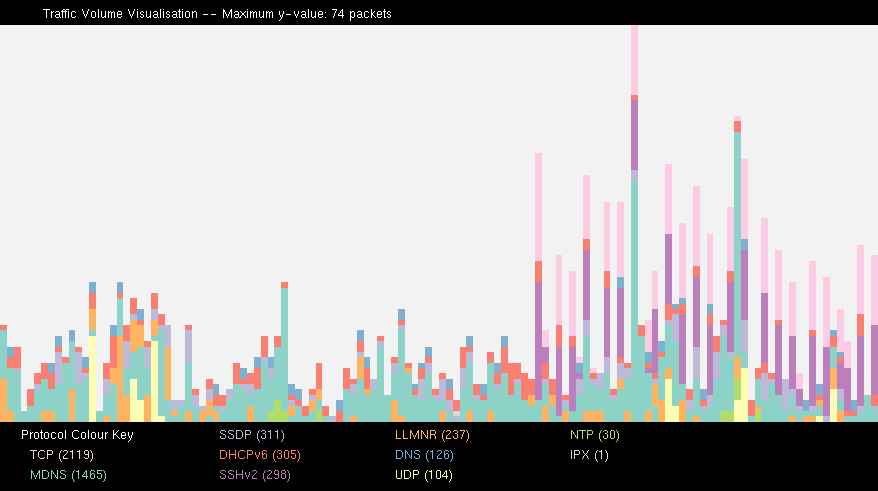
\includegraphics[width=\linewidth]{materials/traffic-volume.png}

The Traffic Volume visualization is inspired by the `FlowScan' graph
\cite{plonka2000flowscan}. The objective is to allow users to see at a glance
if a particular protocol is being exploited in the network. It is realised as a
stacked bar chart which displays the volume of data arriving in each time
interval. Each column is segmented into sections with heights proportional to
the total number of packets transmitted for each protocol.
In addition, the column segments are colour-coded and can be cross-referenced
with a protocol key underneath the visualization.

To help distinguish between different protocols, colours are selected from a
palette which provides colours from a qualitative colour scheme.
The increase in both column height and colour proportion should draw attention
to any protocol which becomes overburdened. For instance, if a network
saturated with TCP traffic suddenly becomes flooded with DNS requests, the
drastic change in colour will alert the user to the change in circumstances.

A control panel is provided in the right panel for adjusting the
number of time intervals displayed at once on the x-axis. The y-axis scales
automatically to fit the current data.
